\documentclass[10pt]{jarticle}
\usepackage{float}
\usepackage{adrobo_abst}
\usepackage[dvipdfmx]{graphicx}
\usepackage{amssymb,amsmath}
\usepackage{bm}
\usepackage[superscript]{cite}
\usepackage{enumerate}
\usepackage{url}
%\usepackage[absolute]{textpos}

\renewcommand\citeform[1]{(#1)}

\begin{document}
    
    \makeatletter
    \doctype{2020年度卒業論文概要}
  \title{カメラ画像と目標方向を用いたEnd-to-End学習によるシナリオに基づくNavigation手法の提案}{(カメラ画像と目標方向による予備実験)}
    \etitle{Making Research Paper}{($\bigcirc\bigcirc\bigcirc$)}
    
    \author{18C1096\hspace{.5zw}春山健太}
    \eauthor{Kenta HARUYMA}
    
    \makeatother
    
    \abstract{When preparing the manuscript, read and observe carefully this sample as well as the instruction manual for the manuscript of the Transaction of Japan Society of Mechanical Engineers. This sample was prepared using MS-word. Character size of the English title is 14 pts of Times New Roman as well as sub-title. The name is 12 pts. The address of the first author and the abstract is 10 pts of Times New Roman. Character spacing of the abstract is narrowed by 0.2 pts preferably.}
    
    \keywords{Mechanical Engineering, Keywords List}
    
    \maketitle
    
    \supervisor{指導教員:林原安男 准教授}
    
    \section{緒\hspace{2zw}言}%===========================
    近年,様々なセンサを用いた移動ロボットの自律移動に関する研究が盛んに行われており,
    その中でカメラ画像を用いてロボットへ自律移動を行わせる研究も行われている.
    Bojaskiら\cite{nvidia}は人間のハンドル操作によるステアリングの
    角度の模倣学習を行い,画像を用いて走行を行う方法を提案している.

    また岡田ら\cite{okada}はLiDAR, オドメトリ
    などを入力とするルールべースの制御器を用いて自律移動を行い,
    その制御器の角速度とロボットに取り付けたカメラ画像を用いて
    学習器の訓練を行い,学習後はカメラ画像のみを用いて自律移動を行う.
    ルールベース制御器を用いることでデータセットを自動的に収集し,
    その経路追従行動を模倣する手法を提案している.
    上記の研究により,カメラ画像を用いてロボットが一定の経路を周回することが可能であると示されている.
    
    次に,走行する経路を一定から拡張について考える.
    経路内に\reffig{bunki}のような分岐路が含まれる場合に,
    赤で示す「直進」と緑で示す「左折」の経路を選択するためには
    カメラ画像のみでは情報が不足していると考えられる.
    そのため,データセットへカメラ画像以外に「直進」「右折」「左折」の目標とする方向の情報
     ( 本研究では”目標方向”とする )を追加することで分岐路において特定のルートを選択できる可能性がある.

    そこで,カメラ画像と目標方向を入力とする学習器の出力を用いた走行において,目標方向によって
    分岐路で任意のルートへ走行経路を変更が可能であるかの検証を行う.
    \begin{center}
        \begin{figure}[h]
            \centering
            \includegraphics[width=0.3\textwidth]{./fig/bunki.pdf}
            \caption{Cross road}
            \label{fig:bunki}
        \end{figure}
    \end{center}
    % 本稿では,研究概要作成に関する主な原稿体裁をまとめた.
    
    % 本文には,半角かな文字は使用せず,文章の区切りには全角の読点(,)と句点(.)を用いる.
    
    % \section{記号・単位の書き方}%===========================
    % \begin{table}[!h]
    %     \begin{tabular}{lcl}
    %         $L$ & : & 長さ [m] \\
    %         $t$ & : & 時間 [s] \\
    %         $x$ & : & 流れ方向の座標 [m] \\
    %         $\alpha$ & : & 熱伝達率 [$\mathrm{W/(m^2\cdot K)}$] \\
    %         $Re$ & : & レイノルズ数 \\
    %         $\bm{R}$ & : & 回転行列 \\
    %         $\bm{t}$ & : & 並進ベクトル \\
    %     \end{tabular}
    % \end{table}
    
    % 量記号はイタリック体,単位記号はローマン体,無次元数はイタリック体で書く.
    % 数学記号・単位記号及び量記号は,半角英数字を使用する.単位は,SI単位を使用し,4~MPa のように書く.
    
    % 分野によって作法は異なるが,わかりやすさの観点から行列の表記は大文字のイタリック体・ボールド体を推奨し,ベクトルの表記は小文字のイタリック体・ボールド体を推奨する.
    
    % \section{見出しの書き方}%===========================
    
    % 論文の章立ては.章・節・項である.章見出しはゴシック体で記述し,2行分をとって行の中ほどに書く.
    % 18字以上は3行分を必要とするが,見出しが不必要に長くなるのは推奨されない.
    
    % \subsection{節の書き方}
    
    % 項の見出しもゴシック体で記述し,本文は見出し後に改行をせずに,直後に2文字分の空白を空けてから書き始める.
    
    \section{提案手法}%===========================
    学習器の訓練を行う「学習フェーズ」,訓練した学習器の出力を用いて走行する「テストフェーズ」
    の2つに分けて述べる
    \subsection{学習フェーズ}
    学習器の訓練を行う学習フェーズで用いるシステムを\reffig{system_learning}に示す.
    地図ベースの制御器はROS Navigation\_stackへ目標方向の
    生成機能を追加する形で作成したルールベース制御器である.
    学習は下記の一連の流れを 1 step として,設定した step 数行う.
    目標方向は「continue」「go straihgt」「go left」「go right」の4つとし,これらを要素数4のOne-hotベクトルで表現する.
    1)LiDAR とオドメトリから得たデータを入力とする地図ベースの制御器の出力を用いて
    自律走行を行う
    2)地図ベースの制御器の出力からヨー方向の角速度と目標方向,機体に取り付けたカメラから RGB 画像を取得し,訓練データへ加える
    3)訓練データを 入力 : カメラ画像,目標方向 目標出力 : 角速度 として学習器の訓練を行う
    4)学習器の出力を記録.
    % \begin{enumerate}
    %     \setlength{\parskip}{0cm} % 段落間
    %     \setlength{\itemsep}{0cm} % 項目間
    %     \item LiDAR とオドメトリから得たデータを入力とする地図ベースの制御器の出力を用いて
    %             自律走行を行う
    %     \item 地図ベースの制御器の出力からヨー方向の角速度と目標方向,機体に取り付けたカメラ
    %     から RGB 画像を取得し,訓練データへ加える
    %     \item 訓練データを 入力 : カメラ画像,目標方向 目標出力 : 角速度 として学習器の訓練を
    %     行う
    %     \item 学習器の出力を記録.
    % \end{enumerate}

    % \begin{table}[h]
    %     \caption{Command}
    %     \label{tab:com}
    %     \begin{center}
    %         \vskip 1zh
    %         \begin{tabular}{|c|c|}
    %             \hline
    %             Target Direction & Data\\ \hline
    %             con & $[100,0,0,0]$ \\ \hline
    %             go straihgt & $[0,100,0,0]$ \\ \hline
    %             go left & $[0,0,100,0]$ \\ \hline
    %             go right & $[0,0,0,100]$ \\ \hline
    %         \end{tabular}
    %     \end{center}
    % \end{table}
    
   
    \begin{center}
        \begin{figure}[h]
            \centering
            \includegraphics[width=0.4\textwidth]{./fig/system_learning.pdf}
            \caption{System of learning}
            \label{fig:system_learning}
        \end{figure}
    \end{center}
    
    \subsection{テストフェーズ}
    設定した step 数に達した場合に, \reffig{system_test}に示すように地図ベースの制御器の出力による
    動作から,中央のカメラ画像と目標方向を入力とした学習器の出力による動作へ切り替えて走
    行を行う.テスト時の目標方向は Joy stick コントローラのボタンを用いて入力する.
    テストフェーズにおける手順を下記に示す
    1)機体に取り付けた中央のカメラから RGB 画像 ,Joy stick コントローラより目標方向の
    データを取得
    2)取得したデータ ( カメラ画像,目標方向 ) を学習器へ入力
    3)学習器の出力(角速度)をモータへ与える
    % \begin{enumerate}
    % \setlength{\parskip}{0cm} % 段落間
    % \setlength{\itemsep}{0cm} % 項目間
    % \item 機体に取り付けた中央のカメラから RGB 画像 ,Joy stick コントローラより目標方向の
    % データを取得
    % \item 取得したデータ ( カメラ画像,目標方向 ) を学習器へ入力
    % \item 学習器の出力(角速度)をモータへ与える
    % \end{enumerate}
    \begin{center}
        \begin{figure}[h]
            \centering
            \includegraphics[width=0.38\textwidth]{./fig/system_test.pdf}
            \caption{System of test}
            \label{fig:system_test}
        \end{figure}
    \end{center}
    
    \section{実\hspace{2zw}験}%===========================
    実験はシミュレータ上で行い,
    環境はGazebo上で作成した\reffig{bunki}で示す道幅が2.5mの十字路とし,
    使用するロボットはturtlebot3 waffleへカメラを3つ追加したモデルを用いる.
    実験条件は「壁に衝突せず,目標方向に対応したコースを選択」を成功,
    「目標方向とは異なったコースを選択する,または壁に衝突」を失敗とする.
    目標方向は学習フェーズ,テストフェーズともに
    図中の緑ー青間を「continue」青ー1「go straihgt」青ー2「go left」青ー3「go right」
    を入力している.
    step数は4000[step]行った.
    実験結果を\reftab{suc}に示す
    % \begin{enumerate}
    %     \setlength{\parskip}{0cm} % 段落間
    %     \setlength{\itemsep}{0cm} % 項目間
    %     \item 学習フェーズによって,学習器の訓練 ( 経路の学習 ) 行う
    %     ( 制御:地図べースの制御器の出力 )
    %     \item 設定した step 数を学習後,訓練フェーズへ移行
    %     ( 制御:学習器の出力 )
    %     \item コース内に設定した地点において目標方向のコマンドを入力,挙動を確認
       
    % \end{enumerate}
    \begin{center}
        \begin{figure}[H]
            \centering
            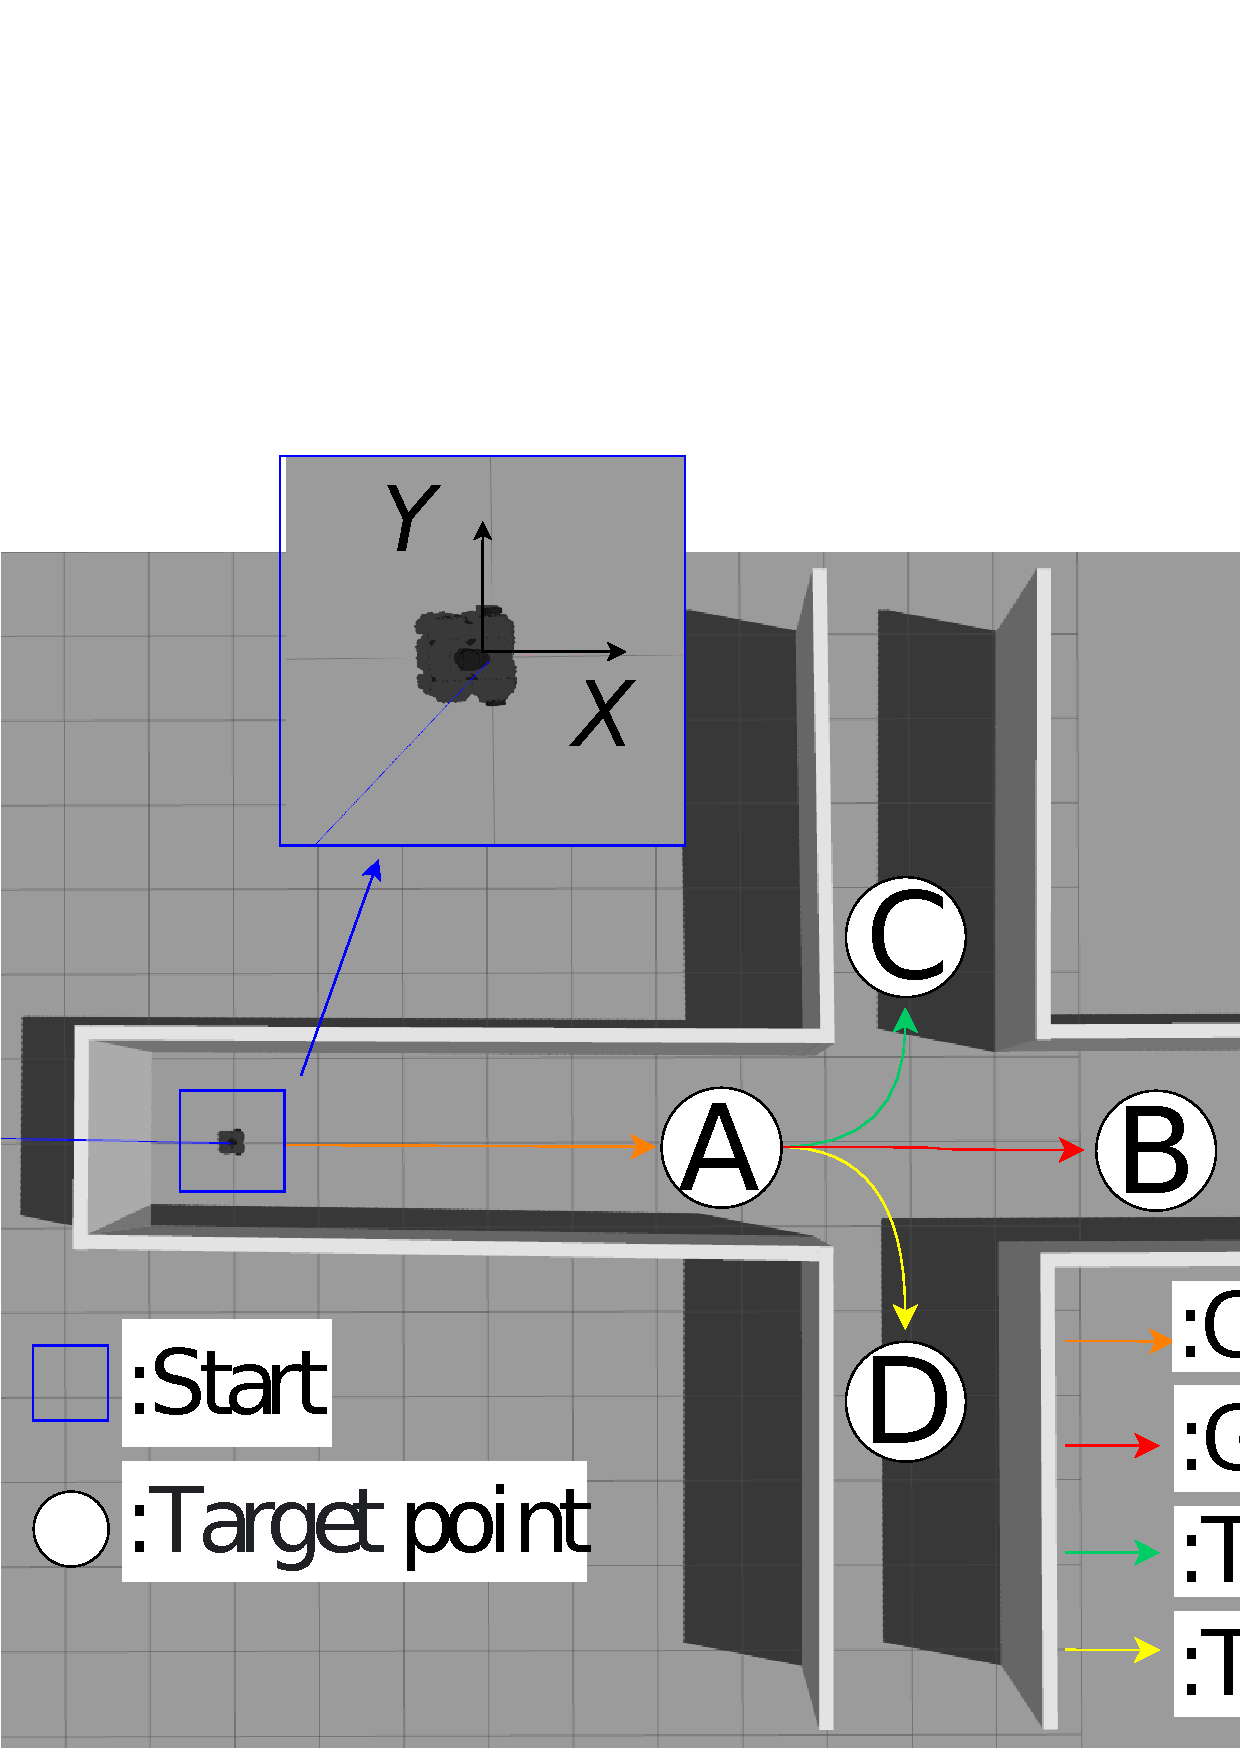
\includegraphics[width=0.35\textwidth]{./fig/zyuziroute.pdf}
            \caption{Route of }
            \vskip 0.1zh
            \label{fig:exp}
        \end{figure}
    \end{center}
    \begin{table}[H]
        \caption{suc}
        \label{tab:suc}
        \begin{center}
            \vskip 0.1zh
            \begin{tabular}{|c|c|}
                \hline
                Point & Number of successes\\ \hline
                $1$ & $5/5$ \\ \hline
                $2$ & $4/5$ \\ \hline
                $3$ & $5/5$ \\ \hline
            \end{tabular}
        \end{center}
    \end{table}
    
    % \section{数式の書き方}%===========================
    
    % 式番号は,式と同じ行に右寄せして( )の中に書く.また,本文で式を引用するときは,\refeqn{sample-eq1}のように書く.
    % \begin{equation}
    %     \gamma(t) = \frac{ji}{N} \label{eq:sample-eq1}
    % \end{equation}
    % \begin{equation}
    % \bar{C}(t)=\frac{1}{N}\sum_{i=1}^{N}C_i(t) \label{eq:sample-eq2}
    % \end{equation}
    
    %\begin{table}[!b] \notag
    %\begin{minipage}{\textwidth}
    %\begin{tabular*}{\textwidth}{@{\extracolsep{\fill}}lr}
    %{\footnotesize
    %$\displaystyle 
    %u^*_{i,j} = u^n_{i,j} - \Delta t \left\{u^n_{i,j}\frac{u^n_{i+1,j} - u^n_{i-1,j}}{2\Delta x} + v^n_{i,j}\frac{u^n_{i,j+1} - u^n_{i,j-1}}{2\Delta y} + \frac{1}{Re}\left(\frac{u^n_{i+1,j} - 2u^n_{i,j} + u^n_{i-1,j}}{(\Delta x)^2} + \frac{u^n_{i,j+1} - 2u^n_{i,j} + u^n_{i,j-1}}{(\Delta y)^2}\right) \right\}
    %$}
    %& $\inlineTag\label{eq:long-eq} $
    %\end{tabular*}
    %\end{minipage}
    %\end{table}
    
    % 式を書くときは,2文字分空白を空ける.
    % また,必要行数分を必ず使うようにして書く.
    % 3行必要とする式を2行につめて書いたり,2行に分かれる式を1行に収めたりしない.
    % なお,本文と式,式相互間は1行以上の空白を空けて,見やすくする.
    % ポイント数は本文に準じるものとするが,添え字等が小さく読みにくくなるときは適宜拡大する.
    
    %式はなるべく片側に書くことが望ましいが,両側にまたがる場合は,読む順序に混乱を生じないように,そのページの式の上,または下の本文全部を両方にまたがるように書かなければならない.
    %本見本では\refeqn{long-eq}のようにページの最上段もしくは最下段に配置している場合は,上記のような混乱は生じ得ないので以下の文章は2段組で続けることができる.
    %ただし,所望の位置に表示されない,文字が重なるなどレイアウト上の多くの問題が生じるため,極めて推奨しない.
    
    % \section{引用文献の書き方}%===========================
    % 本文中の引用箇所には,右肩に小括弧をつけて,通し番号を付ける.例えば,文献\cite{工大2005}や,文献\cite{Shibutani2004, Handbook1979, Kikuchi2017, Adrobo2019}のようにする.
    
    % 引用文献は,英文で記述されているもの(文献\cite{Shibutani2004}など)は英文で書き,本文末尾に引用順にまとめて書く.専門的な書籍(文献\cite{Handbook1979}など)についても引用しても良い.
    % Web上の資料を引用する場合,例えばオンラインジャーナルなどの場合は文献\cite{Kikuchi2017}のように,webページの場合は文献\cite{Adrobo2019}のように,それぞれ参考文献として記載して引用する.この時,URLとともに参照日を記載すること.ただし,webページの場合は個人の技術ブログなどのように第3者による十分な審査が行われていないものの引用は行ってはいけない.公的な機関が発行しているページであっても,その永続性の問題から必要最小限に留めることを推奨する.
        
    \section{結\hspace{2zw}言}%===========================
    本稿ではカメラ画像と目標方向¥¥¥¥を行い,
    実験結果から
    分岐路において目標方向を用いて特定のルートが選択する行動が見られた.
    
    \vspace{5truemm}
    {\footnotesize
        \begin{thebibliography}{99}
            
            % \bibitem{工大2005}
            % 工大太郎: ``ロボットのしくみ'', 
            % 日本機械学会論文誌A, 
            % Vol.~108, No.~1034 (2005), pp.~1--2.
            
            \bibitem{okada}
            岡田眞也, 清岡優祐, 上田隆一, 林原靖男:``視覚と行動の end-to-end 
            学習により経路追従行動をオンラインで模倣する手法の提案''
            SICE-SI2020予稿集,1147--1152,制御学会SI部門講演会(2020)
            
            \bibitem{nvidia}
            Mariusz Bojarski et al:``End to End Learning for Self-Driving Cars'',
            arXiv: 1604.07316,(2016)
            % \bibitem{Shibutani2004}
            % Y. Shibutani: ``Heinrich's Law Resulted Pattern Dynamics --Part2--'',
            % Proceedings of the 79th Kansai Branch Regular Meeting of the Japan Society of Mechanical Engineers,  
            % No.~04--05 (2004), pp.~205--206.
            
            % \bibitem{Handbook1979}
            % The Japan Society of Mechanical Engineers ed.: ``JSME Date Handbook: Heat Transfer'', 
            % (1979), p.~123, The Japan Society of Mechanical Engineers.
            
            % \bibitem{Kikuchi2017}
            % K. Kikuchi, M. Miura, K. Shibata, J. Yamamura: ``Soft Landing Condition for Stair-climbing Robot with Hopping Mechanism'', 
            % Journal of JSDE, Vol.~53, No.~8 (2018), pp.~605--614, \url{https://doi.org/10.14953/jjsde.2017.2774}.
            
            \bibitem{navigation}
            ros-planning, navigation: 
            \url{https://github.com/ros-planning/navigation}, 
            (参照日 2020年12月30日). 
            
        \end{thebibliography}
    }
    \normalsize
    
\end{document}
